% Source for the "lifecycle of a Block" figure (§3.4).
% Build:  pdflatex block-lifecycle.tex  &&  pdftocairo -svg block-lifecycle.pdf block-lifecycle.svg
\documentclass[border=4pt]{standalone}
\usepackage{tikz}
\usetikzlibrary{arrows.meta,positioning,shapes.geometric}
\begin{document}
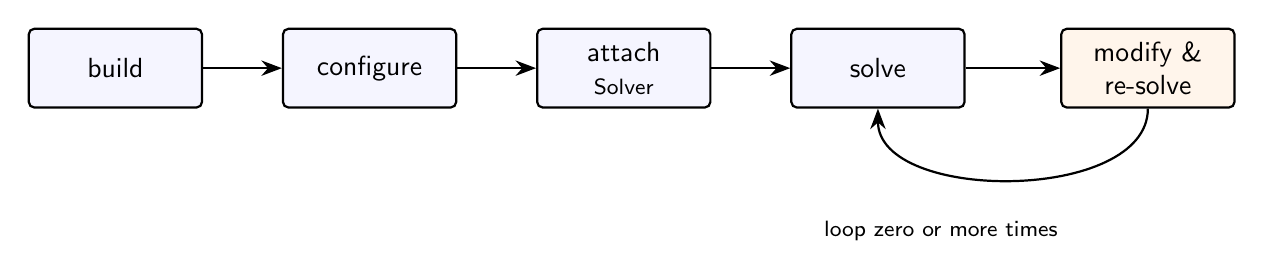
\begin{tikzpicture}[
    font=\sffamily,
    box/.style={draw,rounded corners=2pt,minimum height=10mm,minimum width=22mm,
                fill=blue!4,thick,align=center},
    >={Stealth[length=2.6mm]},
    arr/.style={->,thick}
  ]
  \node[box] (build)  {build};
  \node[box,right=10mm of build]     (config) {configure};
  \node[box,right=10mm of config]    (attach) {attach\\\footnotesize Solver};
  \node[box,right=10mm of attach]    (solve)  {solve};
  \node[box,right=12mm of solve,fill=orange!8] (modify) {modify \&\\re-solve};

  \draw[arr] (build)  -- (config);
  \draw[arr] (config) -- (attach);
  \draw[arr] (attach) -- (solve);
  \draw[arr] (solve)  -- (modify);

  % the modify/re-solve loop back to solve
  \draw[arr] (modify.south) .. controls +(0,-12mm) and +(0,-12mm) .. (solve.south);
  \node[font=\sffamily\footnotesize,below=13mm of solve,anchor=north,xshift=8mm]
       {loop zero or more times};
\end{tikzpicture}
\end{document}
